\subsection{Datenbankentwicklung}
\subsubsection{Systeminstallation}
Um die ArangoDB auf einen Linux Server zu installieren folgt man den Anweisungen auf der Webseite von ArangoDB.

Als ersten Schritt muss ein Repository-Schlüssel dem Paket-Manager \texttt{apt} hinzugefügt werden.
\begin{lstlisting}[language=bash]
curl -OL https://download.arangodb.com/arangodb37/DEBIAN/Release.key
sudo apt-key add - < Release.key
\end{lstlisting}
Anschließend kann über den Paketmanager die Installation folgen:
\begin{lstlisting}[language=bash]
echo 
	'deb https://download.arangodb.com/arangodb37/DEBIAN/ /' | 
	sudo tee /etc/apt/sources.list.d/arangodb.list
sudo apt-get install apt-transport-https
sudo apt-get update
sudo apt-get install arangodb3=3.7.3-1
\end{lstlisting}
Nachdem die Installation abgeschlossen wurde, kann der automatisch gestartete ArangoDB-Services wieder gestoppt werden. Diese Schritte werden nacheinander auf allen vier Nodes im Cluster ausgeführt. \cite{ADB_install}

Um nun einen ArangoDB-Cluster zu starten, haben wir den ArangoDB Starter verwendet. Der Starter ist ein \ac{CLI}-Tool, welches über Parameter die Optionen eines Datenbankservers konfiguriert. 
Für unseren Cluster haben wir für den Hauptserver (Node-4) folgende Konfiguration gewählt:
\begin{lstlisting}[language=bash]
sudo arangodb \
--starter.data-dir=/data/team38 \
--server.storage-engine=rocksdb
\end{lstlisting}
Alle weiteren Nodes wurden mit diesem Befehl mit dem Datenbankserver von Node-4 verbunden:
\begin{lstlisting}[language=sh]
sudo arangodb \
--starter.join c017-node4 \
--starter.data-dir=/data/team38 \
--server.storage-engine=rocksdb
\end{lstlisting}
\citep{ADB_starter}


\subsubsection{Datenmodellierung und Beispielschema}
Um den Use Case für den Graphen so verständlich wie möglich zu gestalten, haben wir uns ein einfaches Schema entschieden. Es besteht aus genau zwei Entitäten. Eine Collection, welche Autodaten enthält und eine weitere Collection, die die Kanten für unseren Graphen enthält. Diese Kanten zeigen von einer Auto-Entität auf eine andere Auto-Entität.
\begin{figure}[htbp] 
  	\centering
     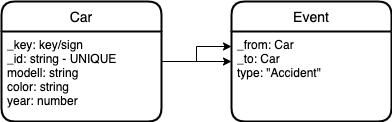
\includegraphics[width=.7\textwidth]{./images/8.Schema.png}
 	\caption{Implementiertes Beispielschema}
  \label{fig:DataSchema}
\end{figure}
\subsubsection{Import der Beispieldaten}
Über das Webinterface der Datenbank lassen sich für jede Collection über ein \ac{JSON}-Import Daten importieren.
Ausschnitt von Car Beispieldaten:
\lstinputlisting[linerange={1-9}, caption=Beispieldaten Auto, label=Beispieldaten Auto]{./json/cars.json}
Ausschnitt von Event Beispieldaten:
\lstinputlisting[linerange={1-9}, caption=Beispieldaten Event, label=Beispieldaten Event]{./json/events.json}
\subsubsection{AdHoc-Anfragen}
\begin{figure}[htbp] 
  	\centering
     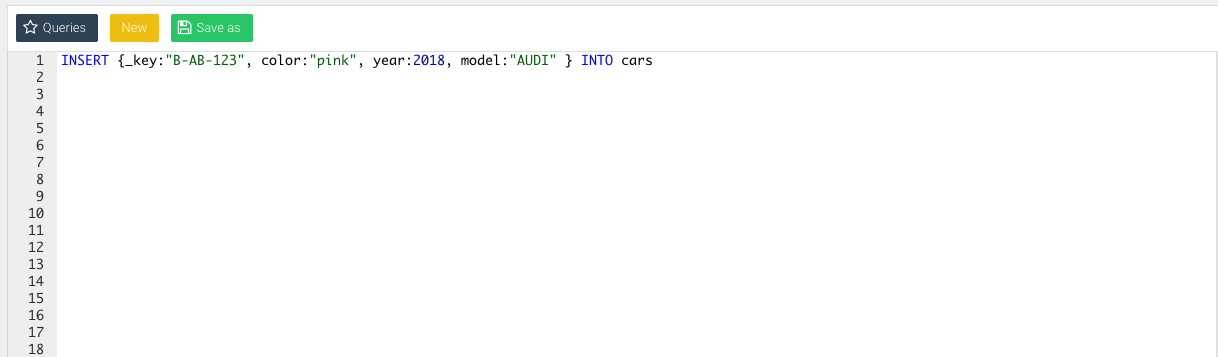
\includegraphics[width=1\textwidth]{./images/8.create.png}
 	\caption{CREATE von Dokument im Schema}
  \label{fig:DataSchema}
\end{figure}
\begin{figure}[htbp] 
  	\centering
     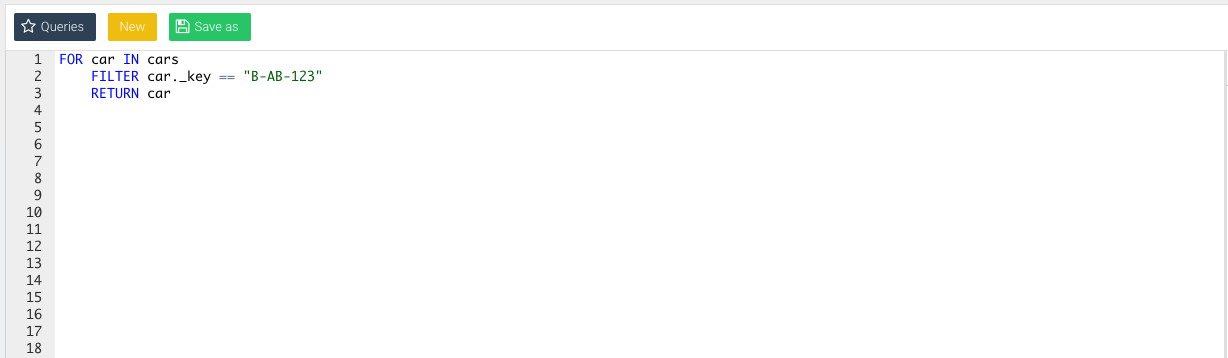
\includegraphics[width=1\textwidth]{./images/8.select.png}
 	\caption{SELECT vom erstellten Dokument}
  \label{fig:DataSchema}
\end{figure}
\begin{figure}[htbp] 
  	\centering
     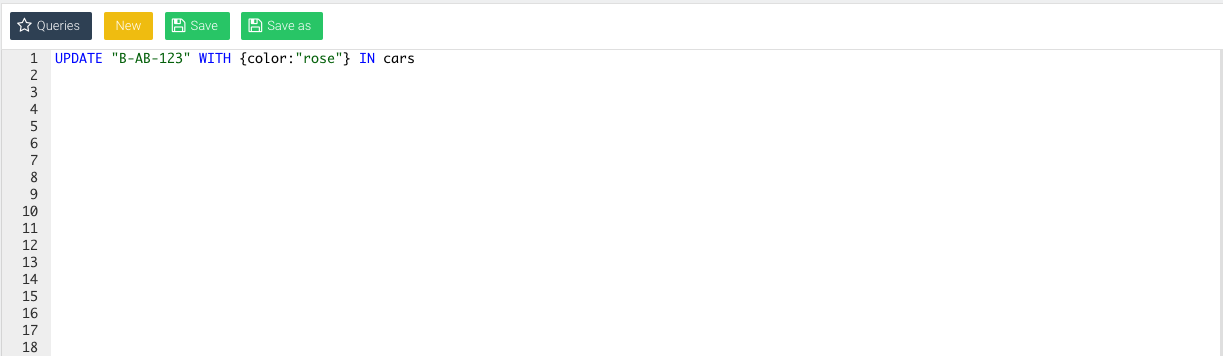
\includegraphics[width=1\textwidth]{./images/8.update.png}
 	\caption{UPDATE vom erstellten Dokument}
  \label{fig:DataSchema}
\end{figure}
\begin{figure}[htbp] 
  	\centering
     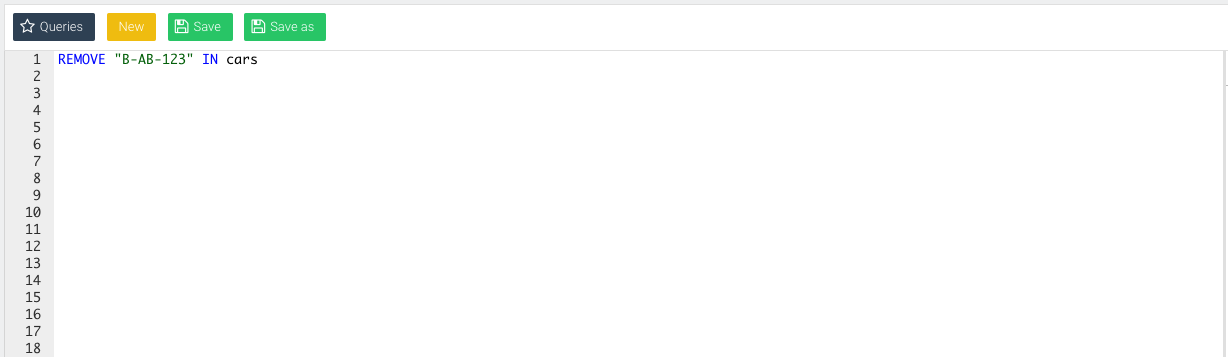
\includegraphics[width=1\textwidth]{./images/8.delete.png}
 	\caption{DELETE vom erstellten Dokument}
  \label{fig:DataSchema}
\end{figure}